\documentclass[fontsize=11pt]{article}

\usepackage{
  amsmath,
  amsthm,
  amssymb,
  graphicx,
  braket
}

\usepackage[hidelinks]{hyperref}
\usepackage{cleveref}

\title{CS 598 DH Final Project}
\author{Yue Chen, Yuxuan Wu}
\date{\today}


\begin{document}
\maketitle


\begin{abstract}
Oblivious RAM (ORAM) is a cryptographic primitive that allows a single client to access an untrusted server while concealing the access patterns, thereby providing stronger privacy guarantees. To go a step further, Oblivious Parallel RAM (OPRAM) introduces a primitive where multiple mutually trusted clients are accessing the same ORAM in a paralleled manner. This introductory project will focus on presenting the main ideas of 3 important OPRAMs that are introduced between 2015-2017. To do so, we will first outline two fundamental ORAMs schemes: Path ORAM and Tree ORAM, followed by the corresponding constructions and implementations of these 3 OPRAMs. In the end, we will briefly touch on some newer papers in the OPRAM field and some possible applications that may develop upon it.
\end{abstract}

\section{Introduction}
\subsection{ORAM}
Oblivious RAM allows a client that has limited storage space to outsource data to an untrusted server. The client is allowed to perform read and write operations while leaking no information about the access pattern, i.e., the pattern should be uniformly random in the server's view. Take figure \ref{fig:access_pattern} as an example, the access pattern can be observed and recorded by the server. Even though the data stored in the server are all encrypted, from the access pattern the server may guess that these data are sorted. We don't want this kind of information to be leaked. The Oblivious RAM scheme helps address this problem. We see these ORAM schemes as compilers that take any program as input, and output a secure program, where the access patterns is obfuscated (See figure \ref{fig:obfuscated}).
This primitive is initially introduced by Goldreich and Ostrovsky \cite{GO96}. Since then, there are many researches on this scheme. The main focus is the bandwidth of client-server communication. 

\begin{figure}
    \centering
    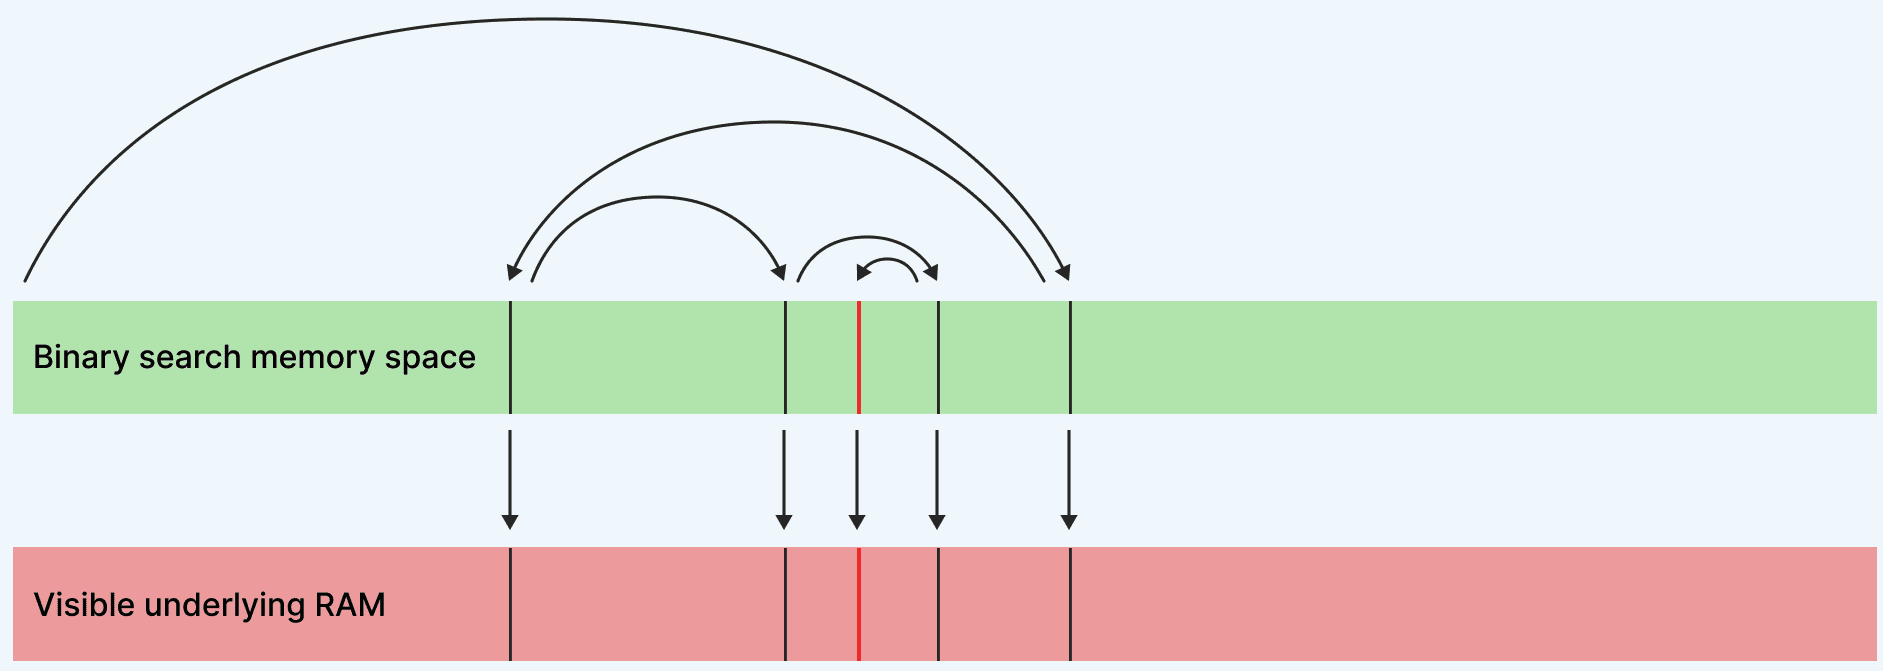
\includegraphics[width=0.5\linewidth]{pics/access_pattern.png}
    \caption{Access patterns leak information.}
    \label{fig:access_pattern}
\end{figure}
\begin{figure}
    \centering
    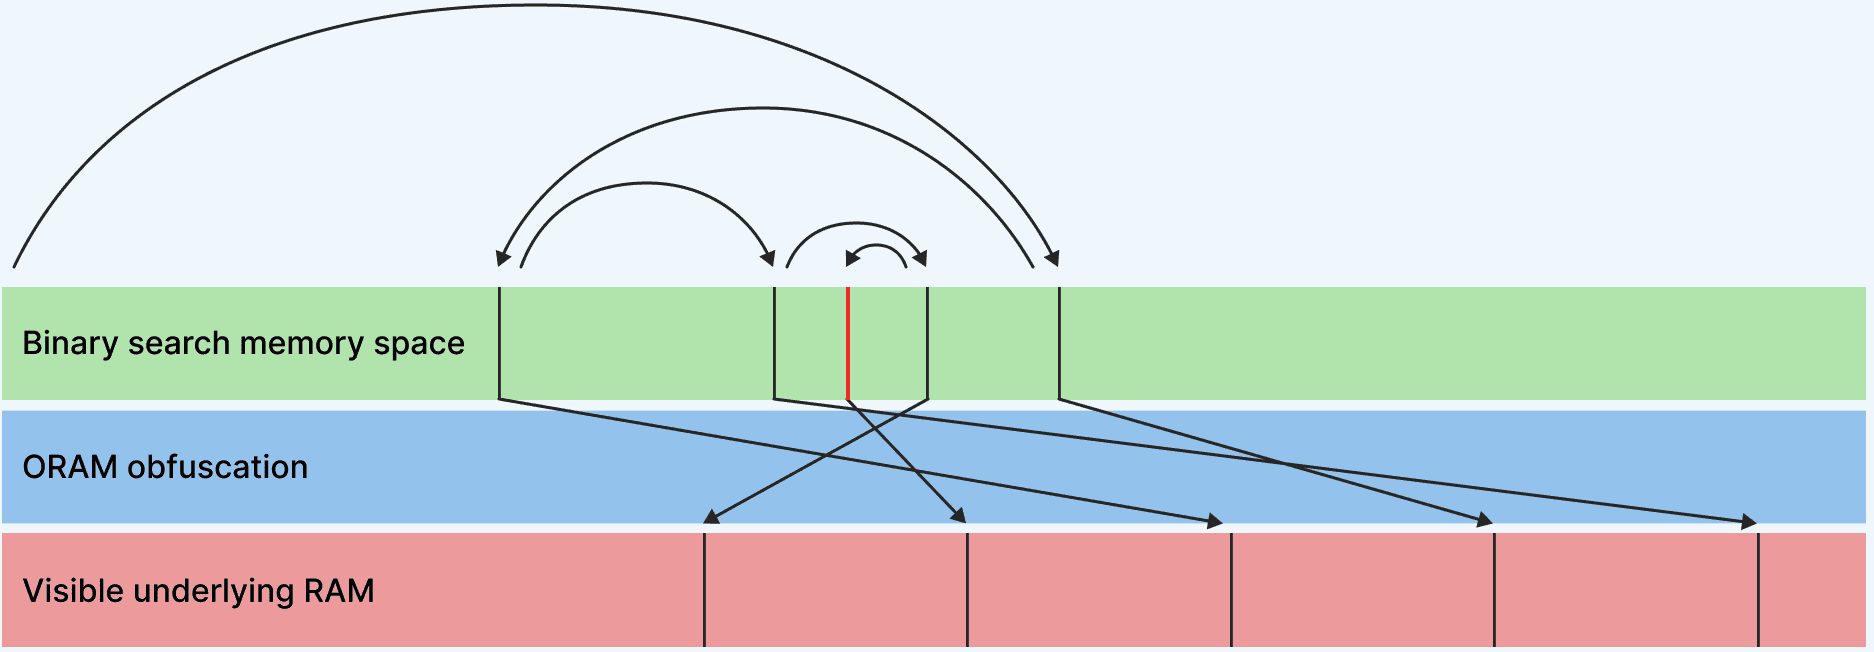
\includegraphics[width=0.5\linewidth]{pics/obfuscated.png}
    \caption{ORAM obfuscates access pattern.}
    \label{fig:obfuscated}
\end{figure}






In the work of Goldreich and Ostrovsky, they have shown that ORAM scheme has a lower bound $\Omega(\log n)$ amortized bandwidth blowup, where $n$ is the size of the database. The ``bandwidth blowup" is the ratio of the bandwidth required for an ORAM access to the bandwidth required for a normal RAM access. Later, in 2018, the paper OptORAMa: Optimal Oblivious RAM \cite{OptORAMa18} gives a theoretical optimal ORAM scheme that achieves a $O(\log n)$ amortized bandwidth blowup. 
 To help understand the Oblivious Parallel RAM schemes better, we will introduce the high-level idea of two important ORAM schemes in section 2.1 and 2.2.


\subsection{OPRAM}
A limitation on ORAM schemes is that they only allow a single client to perform computation on one server. However, we also want to explore the possibilities to run parallel programs in a secure scheme as parallelism helps increase the throughput of some computations. Parallel RAM schemes combine the advantages of both RAM and the circuits models: RAM supports random access but is naturally sequential; circuit models give the power for parallelism, but do not support random access. The Oblivious Parallel RAM schemes are compilers that upgrade PRAMs schemes. It allows $m$ mutually trusted clients to outsource data on one untrusted server while hiding all the access patterns. 

One naive approach for this OPRAM compiler is to run ORAM schemes sequentially, in which the untrusted server processes ORAM querying requests one after another. The approach is correct but far from being efficient, since it requires only one request to be taken at the same time. To improve based on that, researchers have been seeking different methods to introduce parallelism into the ORAM schemes, as the server is powerful enough to handle multiple requests parallelly.

Instead of running ORAMs sequentially, we want to upgrade ORAM so to run them in parallel. The main challenge is to deal with data collisions in plain ORAM schemes that need serial execution.. To ensure both correctness and obliviousness, whenever multiple clients want to operate on the same address, the OPRAM scheme must provide a solution to resolve conflicts while not revealing any new information. The concept of OPRAM is initially introduced by Boyle, Chung and Pass \cite{BCP16}. In their work, they upgraded the Tree ORAM scheme with $O(\log^3 n)$ client-server bandwidth blowup. This work was latter improved by Chen, Lin, and Tessaro to reach a $O(\log^2 n)$ amortized client-server bandwidth blowup, and a $O(f(m)\log m \log^2 n)$ parallel runtime blowup \cite{CLT16}, where $f(m) = \omega(1)$. The parallel runtime blowup is further cleaned up by Nayak and Katz \cite{NK16}. They removed the term associated with the client number $m$, reducing the blowup to $O(\log^2 n)$. There are many other excellent works in this field \cite{CS17, CNS18, OptOPRAM20}, but we will only cover the first three papers for a basic introduction to OPRAM schemes.

\section{Preliminaries}

These three papers we focus on are all based on Oblivious RAM schemes. In ORAM, one client wants to store $N$ data cells (also called blocks) on the server. Each cell is $B$ bits wide. All the data stored on the server is encrypted to prevent the server from observing the plain text. We give logical address $addr \in \set{1, \ldots, N}$ to all the $N$ data cells. The client can use $\operatorname{Access}(\operatorname{op}, addr, v)$ to read and write data, where $\operatorname{op} \in \set{ \text{READ}, \text{WRITE}}$, and $v = \bot$ if $\operatorname{op} = \text{READ}$. 

\subsection{Tree ORAM}
The Tree ORAM scheme uses a perfect binary tree as the data structure in the database \cite{CP13}. Let $N$ be the number of data cells in this tree. Each node of this tree is a bucket that stores $Z = \Omega(\log N)$ many cells. Notice that the path from the root node to any leaf node is unique. Therefore, in order to keep track of the position of each cell, the client locally maintain a position map that records the mapping relationship of every cell to its leaf node. Specifically, for the cell $c$, $pos = \operatorname{Pos}(c)$ calculates the leaf node associated with this cell.  For deeper understanding of bucket size, block/cell size, and tree structure, we refer the readers to \cite{SCSL11, CP13, Path18}. 

We give a high-level idea of the access procedure in non-recursive Tree ORAM: 
\begin{enumerate}
    \item \textbf{Fetch: } Let $r$ denote the logical address requested by the client. Let $c$ be the cell to be fetched. The client traverses the data tree along the path that corresponds to the leaf $pos = \operatorname{Pos}(c)$. For every cell along the path, the client makes exactly one read and one write. If the content is not wanted, then the client writes the value back unchanged (\textit{notice that even if the content is unchanged, there are techniques to re-encrypt the content so that it looks different for the server}). If the cell $c$ is found, then the client writes a dummy value ($\bot$) so to erase the value from this position. Denote the cell $c_{\text{old}}$.
    \item \textbf{Update Position Map: } Randomly choose a new position $pos^\prime \gets [N]$. Update the position map $\operatorname{Pos}(c) = pos^\prime$. By doing this, the new position of this cell is independent from the old position.
    \item \textbf{Put Back: } When the client wants to put the data back to the server, the cell must be put back to the root of this tree. It is not safe to put the data back in any other places because the powerful server may observe and remember the old and new paths, which reveals some information about the access pattern. 
    \item \textbf{Flush:} Pick another random position $pos^* \gets [N]$ and traverse the tree along the path to $pos^*$. For every cell along the path $c_a$ that is assigned to $pos^{\prime \prime}$, we try to push down the cell along the path to $pos^*$ while keeping $c_a$ stay on its own path. This can be done by reading and writing exactly once for every cell in every node along the path. 
\end{enumerate}

In this non-recursive Tree ORAM scheme, the client stores a position map that has size $O(n)$ locally. The common trick to reduce this size to constant is to offload the position map to the server recursively. One can think of the retrieval of the position map as many others call the same ORAM scheme, using the same tree. This is similar to the trick used in storing multilevel page tables in operating systems. 


\subsection{Path ORAM}
Path ORAM is also using a tree data structure on the server \cite{Path18}. This scheme requires a $O(\log N)$ local stash for storing data cells. The key difference between Path ORAM and Tree ORAM is the client-server communication in the \textbf{fetch}, \textbf{put back}, and \textbf{flush} steps. Instead of processing the cells one at a time, Path ORAM performs a cleaner batch-like operation for these two steps. 

When the client traverses the path in the \textbf{fetch} steps, instead of performing read and write exactly once for every data cell, all the path is read and stored to the client's local stash. 
Path ORAM also combines \textbf{put back} and \textbf{flush} together to a single \textbf{eviction} step. Instead of putting a single cell to the root and flushing along the new position $pos^*$, the client traverses the tree from leaf $pos^*$ to the root and tries to write cells in the local stash to the tree while maintaining their original path invariant. 

This operation has the same result as the Tree ORAM as it pushes the data as far as possible to the leaves. However, using these techniques, the bucket size can be very small. In their experiment, $Z = 4$ bucket size is already enough for a good performance. In these setups, Path ORAM has reached $O(\log ^2 N)$ bandwidth blowup for small block size $B=\Omega(\log N)$. 

\subsection{Parallel RAM (PRAM) Programs}
Since we only focus on the access patterns, now we only consider the read and write functions of Concurrent Read Concurrent Write Parallel RAMs. Suppose we have $m$ many CPUs $C_1, C_2, \ldots, C_m$, which are synchronously working in parallel to access the shared database of size $N$. A PRAM program $\Pi$ provides all the $m$ CPUs specific read / write instructions $\operatorname{Access}_{\text{PRAM}}(\text{op}, addr, v)$ in every round of computation. Each access instruction is defined by: 
\begin{enumerate}
    \item \textbf{READ} from shared memory cell with address $addr$. 
    \item \textbf{WRITE} $v$ to $addr$ if $v \neq \bot$ . 
    \item \textbf{Return} the value retrieved in step 1.
\end{enumerate}

Notice that PRAM is allowing multiple parties to call $\operatorname{Access}_{\text{PRAM}}$ simultaneously. If multiple CPUs receives the WRITE instructions that has same $addr$ during the computation, the conflict is resolved by only allowing the lowest-numbered CPU $i$ to rewrite the data memory. 

We also allow communication between CPUs during the PRAM program. Hence, it is possible for $C_i$ to send a message $C_j$ so to ask for help. $C_j$ can access the memory for $C_i$, and return the value $v_{\text{old}}$ if needed. These internal communications are crucial for the following OPRAM schemes when dealing with address collision.


\section{BCP16}
\subsection{Overview}
Now we start describing the general construction idea of Oblivious Parallel RAM introduced by Boyle, Chung, and Pass. In this paper, they build an OPRAM by allowing multiple clients to run Tree ORAM concurrently while giving clear instructions to clients for any conflicts. There are three major issues to be resolved:

\begin{enumerate}
    \item \textbf{Parallel memory lookups:} In the Tree ORAM scheme, every access has a \textbf{lookup} step. If two clients concurrently access the same data cell in the same tree, they must read the exact same path, revealing information that multiple clients are possibly instructed to access the same cell. One way to maintain obliviousness is to always force all clients to access different paths regardless of the number of collisions. We can simulate the server easily by simply choosing $m$ many independent paths for every \textbf{lookup}, where $m$ is the number of clients. Notice that if multiple clients wish to access different cells that live inside the same bucket, we allow the same path to be traversed and read. There is no address conflict in this case, and it has the same probability distribution as picking $m$ independent paths randomly.
    \item We can see that internal communications are required to resolve these conflicts. The details of instructions on these communications will be shown in the following section.
    \item \textbf{Parallel put-backs: }After all $m$ clients have done their calculation and wish to put data cells back to the server, returning the data to the root node as instructed in the Tree ORAM scheme will likely cause an overflow issue. The root bucket of a Tree ORAM can store $Z = \Omega(\log N)$ many cells. This number can be smaller than $m$. Hence, the idea is to put these cells in lower levels, specifically, they reinsert the cells in level $\log(m)$, at which the number of internal buckets is the same as $m$. By doing this, the expected number of data reinserted at each bucket is 1. And, the probability of overflowing the buckets is negligible.
    \item \textbf{Flushing:} As described in the Tree ORAM, in the \textbf{flush} step, every client chooses a random path and flush. The issue is that clients must traverse along the path and perform read/write for each data cell. For each node they access, we only want one of them to read and write. Again, we will show how every conflict is resolved in the next section. Resolving the conflicts is for maintaining the correctness of this algorithm but not for obliviousness. The paths are chosen independently randomly, and we know how to simulate the server's view. 
\end{enumerate}

\subsection{Internal Communication}
In the \textbf{parallel memory lookups} problem, we see that every client should at least learn something from each other so to collaborate on maintaining the obliviousness. Suppose two clients $C_i, C_j$ wish to access the same address $r$. To avoid this collision, we only allow one of them to access the real value, equivalently, one \textit{representative} must be selected between them. Here, we use a similar technique as in the normal PRAM program: the client with a lower ``id" will perform the real access. We also assume that the server can see the communication pattern among all the clients, hence an oblivious protocol is required. The procedure called \textit{OblivAgg} is used for aggregating data together so that the representative has all the information needed to retrieve data for others (see figure \ref{fig:OblivAgg}). 
\begin{center}\fbox{
\begin{minipage}{.9\linewidth}
\begin{center}
  \textit{OblivAgg}
\end{center}
\textbf{Input:} Each client $C_i$ has input $(\text{op}_i, r_i, v_i)$, where $r_i$ is the address, $v_i$ is the data to be written.\\
\textbf{Output:} Each client $C_i$ receives $(r_i, v)$ if $C_i$ is the representative or $(\bot, \bot)$ otherwise. Here, $v$ is the aggregation of all data chosen, which is equal to the data of the client with the smallest id (among those who wish to write).
\end{minipage}
}
\end{center}
In BCP16, they have shown a protocol for this functionality that runs in $O(\log m)$ rounds. In each round, the message size is $O(\log m  + |v|)$.

\begin{figure}
    \centering
    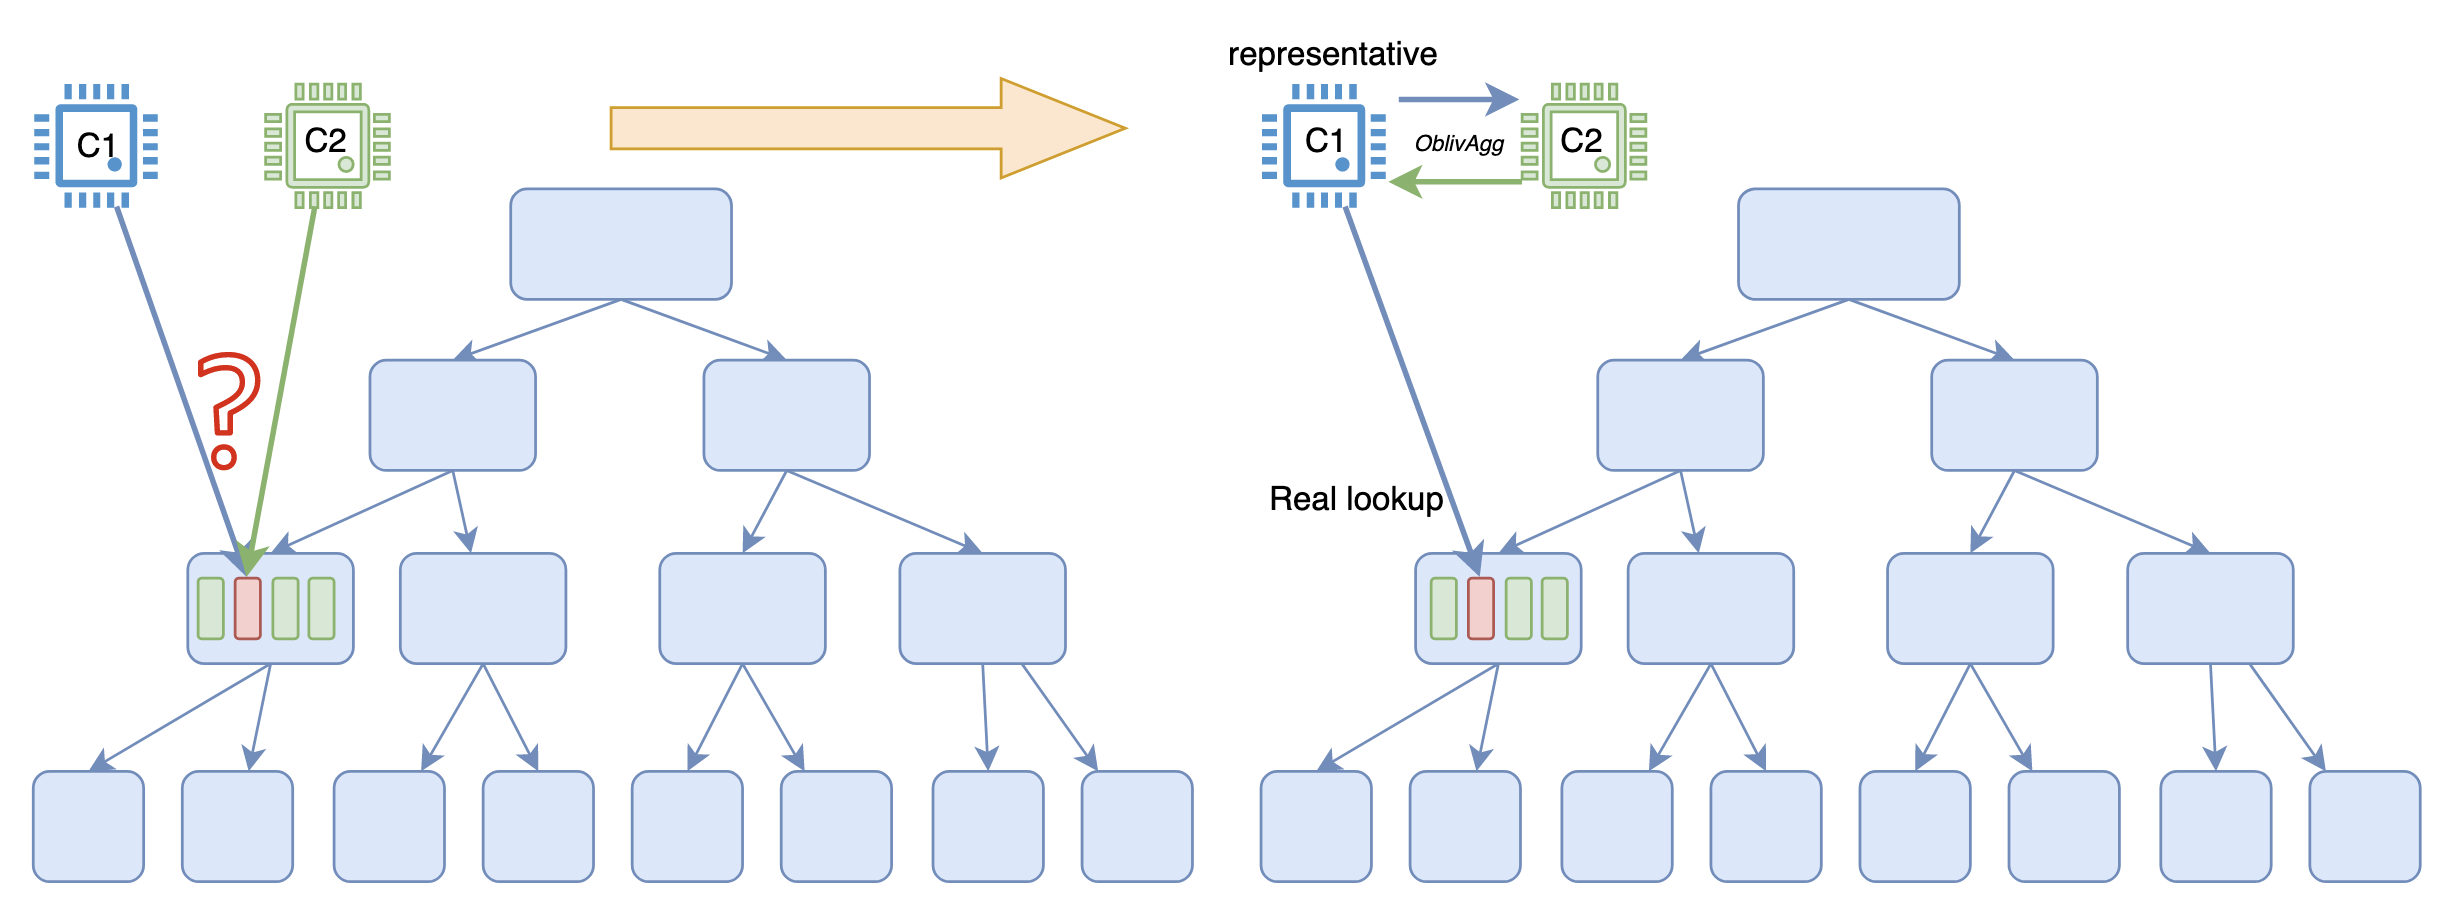
\includegraphics[width=0.75\linewidth]{pics/OblivAgg.png}
    \caption{Oblivious Aggregations resolve conflicts.}
    \label{fig:OblivAgg}
\end{figure}





There is another similar protocol \textit{OblivElect}. This protocol is only in charge of selecting the representative. It will be used in later OPRAM schemes. The key takeaway is that among all the parties that have the same address, then the party with the smallest id writing to that address becomes the representative. If no one writes, then the party with the smallest id reads from the address.\\

After the representative has done the \textbf{lookup} step, it has the responsibility to send the value to other clients who wish to learn the data. Again, this protocol (oblivious multicast) must be oblivious. 

\begin{center}\fbox{
\begin{minipage}{.9\linewidth}
\begin{center}
  \textit{OblivMCast}
\end{center}
\textbf{Input:} The sender $C_i$ has input $(\text{send}, id_i, v_i), id_i \in [m]$, and $v_i$ is the value. Each receiver $C_j$ has input $(\text{recv}, id_j, \bot)$.\\
\textbf{Output:} Each receiver $C_j$ receives output $(id_k, v_k)$, where $id_k = j$.
\end{minipage}
}
\end{center}

For the \textbf{put-back} step, clients must put their updated data back to the server. However, we cannot reveal the information of the destination of each data. Say the client $C_1$ pick some data from path $l_1$, and put it back to the new path $l_1^\prime$. This is an extra information that the server may observe and record, which violates the obliviousness. We need another protocol for hiding the freshly sampled random path. 


\begin{center}\fbox{
\begin{minipage}{.9\linewidth}
\begin{center}
  \textit{OblivRoute$(m, (\text{msg}_i, \text{addr}_i))$}
\end{center}
\textbf{Input:} $m$ is the number of clients. $C_i$ holds message $\text{msg}_i$ to be written to the database at destination $\text{addr}_i$. This $\text{addr}_i$ refers to the address at level $\log(m)$, hence $\text{addr}_i \in [m]$\\
\textbf{Output:} $C_i$ holds $\set{\text{msg}_j : \text{addr}_j = i}$
\end{minipage}
}
\end{center}


\subsection{Technical Ideas}
Now we start describing a simplified non-recursive construction of the OPRAM scheme in this paper \cite{BCP16}. Our goal is to provide a clean high-level idea for this scheme. There are many details in the original paper, but little explanation is given. Consider the following as an explanation of the protocol in the paper. For the inputs of this simplified protocol, we let $r_i$ be the address of cells, and $v_i$ is the data to be written. In the original paper, $r_i$ has a different meaning. But here we stick to the idea of this protocol and only use this cell address. 


\begin{center}\fbox{
\begin{minipage}{0.9\linewidth}
\textbf{Non-recursive-OPAccess($r_i, v_i$)} \\
All clients $C_1, \ldots, C_m$ run this function in parallel. Let $C_i$ be the client who runs the current function.
\begin{enumerate}
    \item Use \textit{OblivAgg} to broadcast $(r_i, v_i)$ and select the representative. If $C_i$ is a representative, it receives the instruction $(r_i, v)$.  Otherwise, it receives $(\bot, \bot)$. Here, $v$ is the aggregated data.
    \item If $C_i$ is the representative, it samples a leaf index $l_i^\prime \gets [L_t]$, where $L_t$ is the number of leaves. Rewrite the position map $\operatorname{Pos}(r_i) = l_i^ \prime$. (This step uses recursion in the original construction.) Non-representative samples a random path for lookup.
    \item Now that we have resolved all access conflicts in step 1, all parties run the following in parallel:
    \begin{enumerate}
        \item \textbf{Lookup: }Traverse the tree along $l_i$ defined in step 2 and read all buckets to local memory. 
        \item Retrieve the old data $v_\text{old}$ at address $r_i$. 
        \item Locally calculate $v_\text{new}$ using both $v_\text{old}$ and $v$.
    \end{enumerate}
    \item Representatives use \textit{OblivAgg} to broadcast the address of cells to be \textbf{deleted} from the database. Then all clients call a sub-protocol $\textit{UpdateBuckets}$ to write local memory back to the original place while removing the old data. 
    \item Representatives use \textit{OblivAgg} to broadcast the address of cells to be \textbf{inserted} to the database. All users use sub-protocol \textit{OblivRoute} to ``reallocate" the data. $C_i$ learns the message set to be inserted. Then it inserts all these data to $\log m$ level on the path $l_i$.
    \item Client $C_i$ randomly sample $l_i^\text{ flush}$ and use \textit{OblivAgg} to share with others. Then, all clients flush the tree in parallel.
    \item Use \textit{OblivMCast} to share the retrieved data $v_\text{old}$.
 \end{enumerate}
\end{minipage}
}
\end{center}

In step 4, the \textit{UpdateBuckets} sub-protocol writes memory cells back to their original places. As this involves writing, the \textit{OblivAgg} helps address conflicts. For step 5, no overflow will occur with overwhelming probability.


\section{CLT16}
\subsection{Overview}
The paper "Oblivious Parallel RAM: Improved Efficiency and Generic Constructions" by T. H. Chan, K. M. Chung, and X. Sun (hereafter referred to as \cite{CLT16}), is widely recognized as an enhanced version of the BCP approach. CLT16 adopts the same structure as BCP, assuming that exactly $m$ clients are communicating concurrently with the outsourced server. Using a concept known as ownership partition, which we will discuss later, CLT16 successfully bypasses the overhead of conflicting path operations. These would otherwise be unavoidable if all the clients shared a single traditional tree-based ORAM.

Recall that in BCP's method, to resolve write conflicts in the put-back stage, each client can only move the data from leaf nodes to the exact $\log(m)$ layer, where $m$ is the number of clients. This approach enables $m$ clients to be directly mapped to $m$ independent subtree structures. It splits the entire tree eviction into isolated, non-interfering subroutines. This allows each client to execute their part of the eviction in the allocated areas simultaneously without blocking one another. Nevertheless, this method still has room for improvement:

\begin{enumerate}
    \item The upper structure of the tree remains unused as it only functions as a search index and doesn't store any valid data.
    \item The mapping relationship between subtrees and clients can be pre-determined, reducing the number of communication rounds needed for clients to know their assigned parts of the tree.
    \item The underlying Tree-ORAM protocol can be replaced with Path-ORAM, which offers the same functionality but with a smaller amortized access bandwidth.  
\end{enumerate}

\begin{figure}
    \centering
    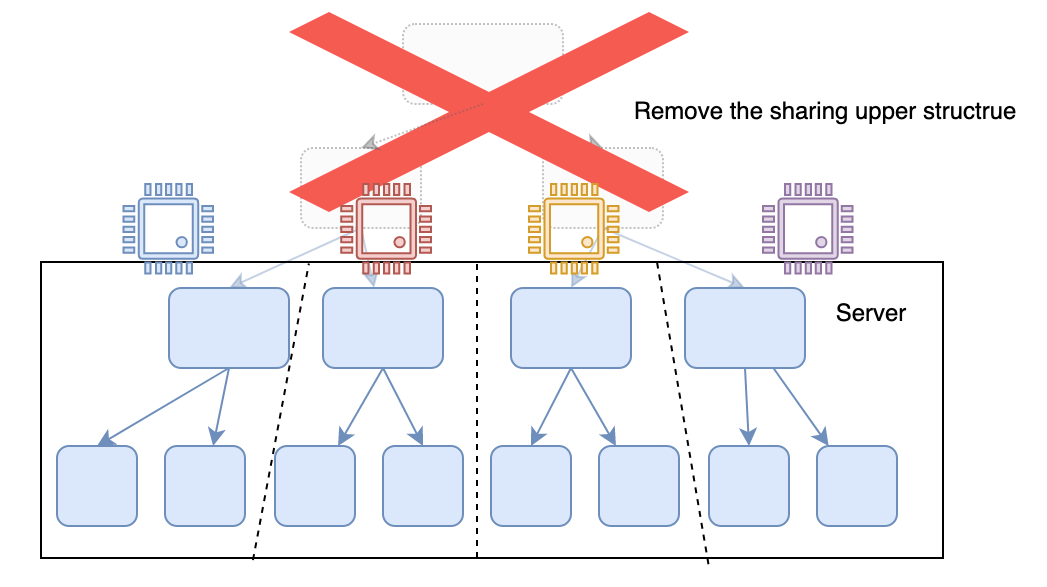
\includegraphics[width=1\linewidth]{pics/ownership_partition.png}
    \caption{Ownership partition with the upper shared structure removed}
    \label{fig:ownership_partition}
\end{figure}

CLT16 addressed these limitations by getting rid of the upper shared structure. By doing this, the rest part of the tree naturally forms a forest of $m$ perfect binary tree, each can be assigned to one client unilaterally responsible for any read or write operations to itself(See Figure \ref{fig:ownership_partition}).

\subsection{Non-recursive Construction of CLT16}

Here, we present a detailed version of the non-recursive construction mentioned in CLT16. The entire protocol organizes the server's storage as $m$ perfect binary trees of equal size. Since the upper layer is removed, each client needs to prepare extra space in their local stash to accommodate the removed storage of size $\log(m)$, which can still be considered constant space given that $m = 2^\lambda$. All clients share a secret key that allows them to communicate in an encrypted manner, and they all have access to the same position map, which not only tells the leaf number of a given cell but also which client is currently accepting access requests to that leaf. The system takes on $m$ requests at a time and continues processing them until all requests are fulfilled before proceeding to the next $m$ requests.

\begin{enumerate}
    \item \textbf{Representative Election.} The clients perform one round of $OblivElect$, where client $i$ inserts its requesting address $a_i$ as the key. Based on the received result, it knows whether it has been selected as a representative. The reason for electing representatives is that in the Path-ORAM scheme, once data is read from an address, the original address becomes invalid since it is shifted to another location. Therefore, the system needs to be aware if any address is read by multiple clients in the same round.
    \item \textbf{Prepare Requests and ``Merge" Requests with the Same Addresses.} Following the previous step, clients naturally form groups where members in the same group want to query the same address, each with a representative assigned(See red flags in Figure \ref{fig:routing-requests}). With only representatives querying the actual address, non-representatives need to perform a dummy request where they randomly decide an address to query and mark their requests as dummy(See the purple arrow in Figure \ref{fig:routing-requests}). This is to keep the request number consistent with the number of clients, otherwise it would be insecure for the outsourced storage since it would learn that some requests have been merged into ones.
    \item \textbf{Route the Request to its Sub-tree Owner.} All clients now have a request to fulfill (either true or dummy). Since they do not necessarily have direct access to the address they are requesting, clients shall route the request to the sub-tree owner (See all the arrows in Figure \ref{fig:routing-requests}).
    \item \textbf{Owners Process the Requests.} From the sub-tree owners' view, all the requests routed to them must have addresses that they should have access to, so they can perform naive Path-ORAM reads, reading the paths from the sub-tree root to leaves for any cells requested. Then, they send the requested cells back to only the requesting representatives. For all the dummy requests they received, they reply with a dummy message.
    \item \textbf{Representatives Broadcast to the Groups.} Upon receiving the requested value, representatives can use \textit{OblivMCast} to broadcast the value to all clients within their group, so that all clients will have the value to perform their operations.
    \item \textbf{Data Reshuffle and Conflict Resolution.} After all clients have finished their operations, the representative gathers all the changes made to the value and resolves any differences in the changes based on some criteria. Representatives then choose a random leaf to put back the value, and adjusts the position map accordingly..
    \item \textbf{Eviction.} This step is similar to steps 3-4. Each representative forwards the changed value to the owners who can only process it. The owners can then in parallel flush the values from their stash to the paths they read in step 4.
\end{enumerate}
Note that the procedure above is round-based. Before all clients have fulfilled their requests, no more requests can be taken by any client, even if they are idle.
\begin{figure}
    \centering
    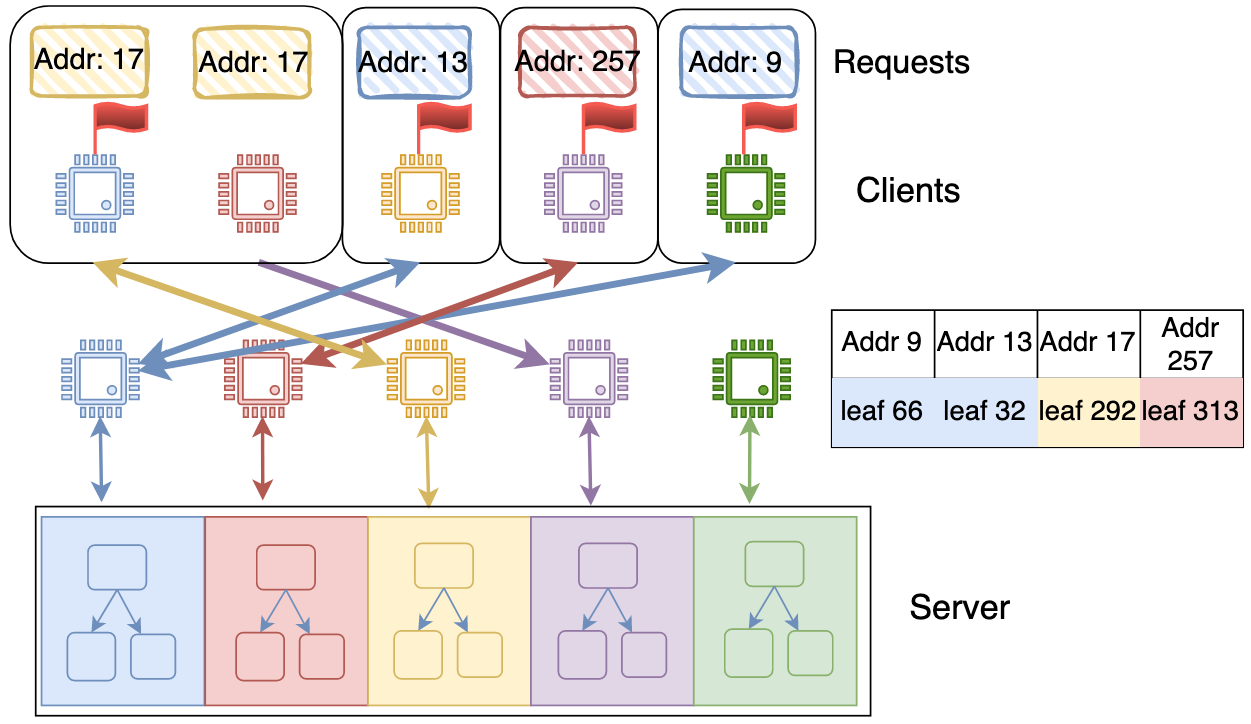
\includegraphics[width=1\linewidth]{pics/route_requests.png}
    \caption{A example of requests routing and representative election}
    \label{fig:routing-requests}
\end{figure}
\subsection{Performance Analysis}
The non-recursive construction above assumes that the communication between clients is inexpensive and can be considered "free". For $m$ requests that the system takes, the communication between clients and servers only happens in steps 4 and 7, which equals $2m$ times of queries. Each query requires an ORAM path traversal that introduces $\log(n)$ bandwidth. Therefore, the total bandwidth between clients and servers is still $O(\log(n))$ under the non-recursive construction.

In the recursive construction, each client needs to perform $\log(n)$ rounds to address the cell. However, each round could still be considered a round of query in the non-recursive construction. Thus, the total bandwidth under the recursive construction for CLT16 is $O(\log^2(n))$.
\section{NK16}
\subsection{Overhead caused by uneven distribution in CLT16}
To prevent clients from modifying nodes they do not own, the construction of the CLT16 requires an additional routing round. In this round, each client looks up the position map and forwards the request to the appropriate owner. To simplify this model, NK16 hereby introduce a famous ``balls into bins" problem to illustrate the potential impact on parallel blowup.

\begin{figure}
    \centering
    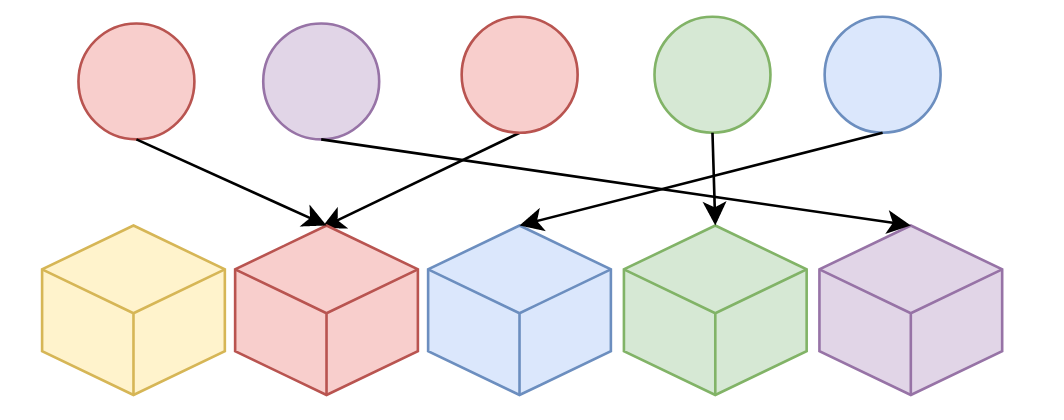
\includegraphics[width=1\linewidth]{pics/balls_n_bins.png}
    \caption{A example of balls into bins assignment}
    \label{fig:balls-n-bins}
\end{figure}

In this analogy, ``balls" represent the requests received by each client, and ``bins" represent the owners who control the path to which the requests belong. Assuming that the incoming requests query completely random addresses, it is possible for two requests to target the same subtree but different addresses(so they won’t form a group and no representative will be elected). In the example of Figure\ref{fig:balls-n-bins}, red bins becomes overloaded as it would need to handle both requests, while this simultaneously starves the yellow bin, which receives no requests for its owned subtree. This phenomenon is more likely than one might expect, in fact, it can be shown that with a high probability, the maximum load among $m$ owners can approximately reach $\frac{\log(m)}{\log(\log(m))} = O(f(m)\log m), f(m) = \omega(1)$. And since the system operates in rounds, idle clients must wait for the most burdened client to finish processing all its queries before the entire system can proceed to the next step. Furthermore, this waiting problem is exacerbated in recursive constructions, where getting the leaf number for a single cell requires performing $\log(n)$ rounds of similar queries.


To address this issue, \cite{NK16} partially delegates the owners' ownership to the clients and allow them to touch the region that they don’t own while not causing conflicts. It suffices to show that this load-balancing approach, proposed by NK16, helps alleviate the waiting issues caused by the uneven distribution.

\subsection{Non-recursive Construction by NK16}
Here, we present a revised construction based on CLT16 and improvements proposed by NK16. The entire protocol, like CLT16, organizes the server's storage into $m$ perfect binary trees of equal size, maintains the same construction of shared secret keys and position map, and processes $m$ requests in a round-based manner.

\begin{enumerate}
    \item \textbf{Representative Election.} The clients perform one round of $OblivElect$, where client $i$ inserts its requesting address $a_i$ as the key, enabling resolution of reads to the same address.
    \item \textbf{Prepare and ``Merge" Requests with the Same Addresses.} Only representatives query the actual addresses. Non-representatives prepare dummy reads to maintain the consistency of the total number of requests with the number of clients.
    \item \textbf{\textit{Read Paths.}} Clients perform their reads in parallel without interfering with each other's operations. Safety is ensured as long as no write operations occur, since reads are non-blocking.
    \item \textbf{\textit{Invalidate Read Cells by Generating a Vector.}} Each client sends an encrypted vector to the server, indicating cells that have been read. This vector, containing mostly ``0s" and a ``1", signals that a cell has been visited. The size of the vector matches the number of cells queried in Step 3.
    \item \textbf{\textit{The Server Performs Additive Homomorphic Encryption.}} Upon receiving $m$ vectors, the server updates the subtrees by adding the vectors to their paths' metadata(See Figure \ref{fig:vector-addition}). The encryption of the vectors ensures the server cannot identify which specific cell has been marked as ``visited."
    \item \textbf{Representatives Broadcast to the Groups.} After receiving the requested value, representatives use \textit{OblivMCast} to broadcast the value to all clients in their group, ensuring all have the necessary data for their operations.
    \item \textbf{Data Reshuffle.} Once all operations are completed, the representative reconciles any differences in the updates made to the value, choose the a random leaf to put back the value, and adjusts the position map accordingly.
    \item \textbf{\textit{Eviction.}} Representatives use \textit{OblivRoute} to forward the updated value to the appropriate owner. Owners then apply reverse lexicographical ordering and choose only one path to flush their local stash, making their best effort. Values not yet put back remain in the owner’s stash.
\end{enumerate} 
\begin{figure}
    \centering
    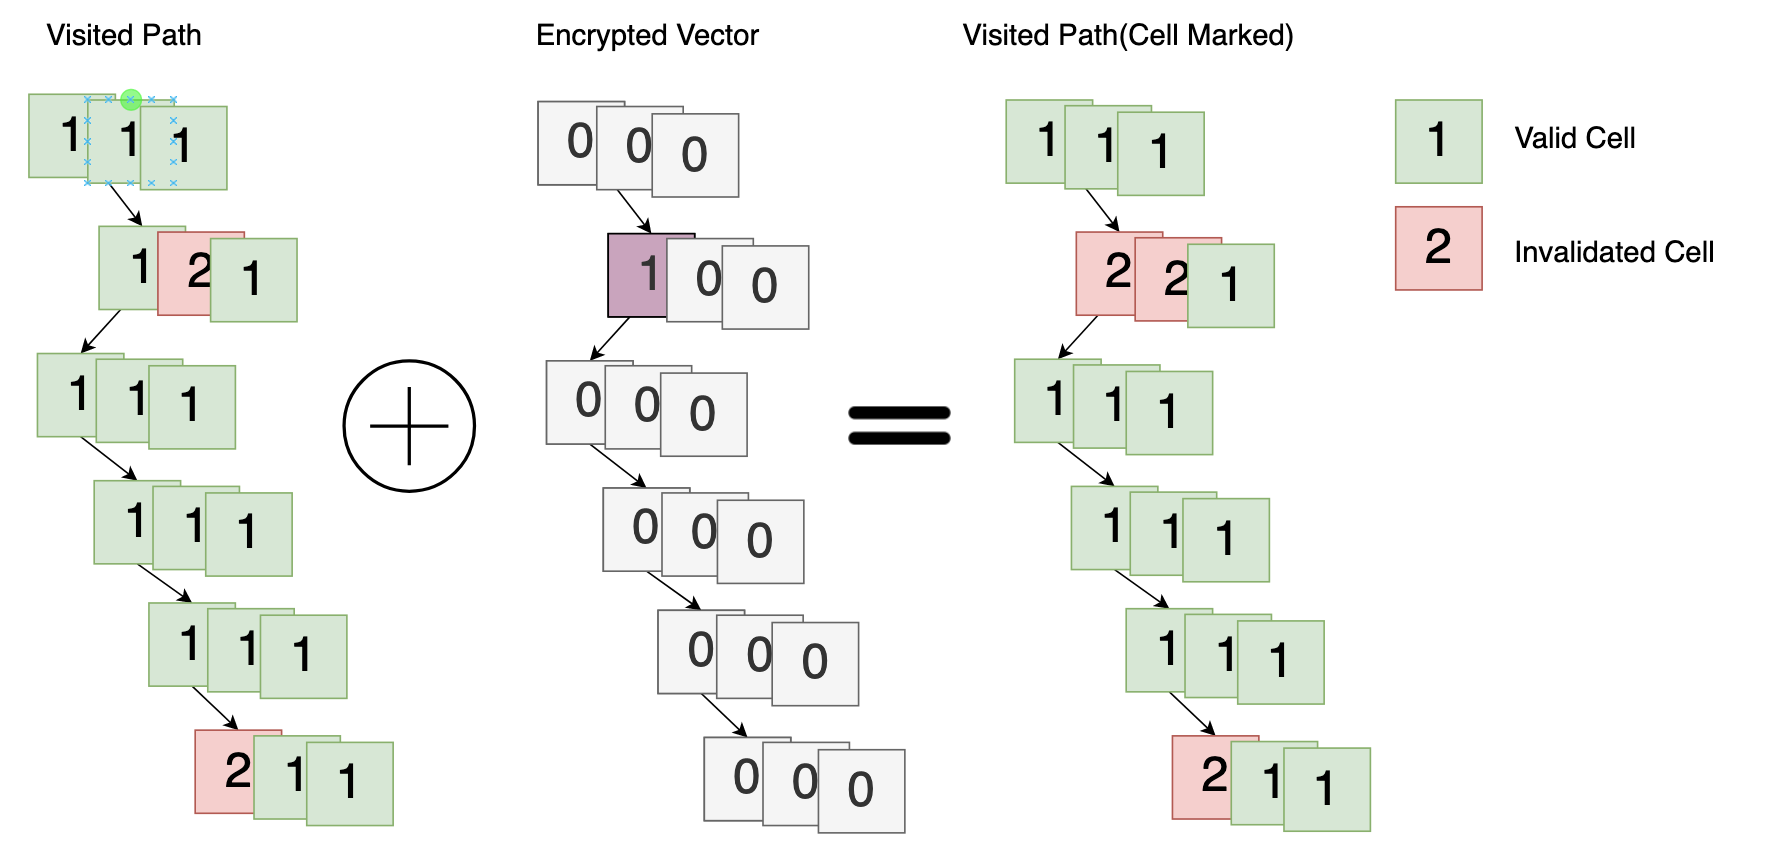
\includegraphics[width=1\linewidth]{pics/AHE.png}
    \caption{Applying Addition for Each Cell to the Visited Path with AHE}
    \label{fig:vector-addition}
\end{figure}
\subsection{Performance Analysis}
There are only three different stages during which clients need to communicate with the server:
\begin{enumerate}
\item \textbf{Path Read:} This stage is conducted in parallel by clients who initially hold the requests. While some clients perform dummy reads, each client must complete exactly one round of path reading so it's load-balanced.
\item \textbf{Mark Visited Cells:} Clients generate vectors of the same size, with each vector marking which cells have been invalidated, thus is load-balanced. Note that the task of adding these vectors is outsourced to the server.
\item \textbf{Eviction:} After values have been transferred to the appropriate clients, each client performs eviction on only one path and is therefore load-balanced.
\end{enumerate}
Thus, the workload is balanced across different clients, where each engages in a constant number of rounds (three) of communication with the outsourced server. Consequently, the parallel runtime blowup removes the term associated with $m$ in CLT16’s scheme. I.e., parallel runtime blowup is improved from $O(f(m)\log(m)\log^2 n)$ to a clean $O(\log^2 n)$, while not changing the bandwidth blowup.


\section{Summary}

Now we have reviewed the first three Oblivious Parallel RAM schemes. 
From BCP's paper, we see how they managed to upgrade Tree ORAM to a simple OPRAM scheme by addressing all possible conflicts. We also see how the structure of the tree can be simplified by Chen \textit{et al}. Their scheme not only reduces the conflicts by partitioning the tree to $m$ parts, but they also use a more practical Path ORAM scheme as a base ORAM protocol, further reducing the bucket size and improving the practicability of OPRAM. In NK16, even smarter tricks are used to reduce the idle time of all clients. 

There are no well-known tools or software packages from our research that explicitly market themselves as utilizing OPRAM. This could be partially because OPRAM is still a relatively primitive research area and has not become a widely known technology, but also because of the difficulty of implementing and maintaining an actual OPRAM protocol. However, we have observed a few frameworks such as Intel SGX and ARM TrustZone, which provide an isolated abstraction(enclave or Trusted Execution Environment) to protect data access from either untrusted operation systems or applications, and we assume these frameworks might be the ones where the concept of OPRAM might be adapted first.


Other interesting topics that are not covered in detail include OPRAM variants under different constructions. We would like to particularly mention some of them: The work of \cite{OptOPRAM20} that introduces an optimal OPRAM scheme utilizing a hierarchical structure to achieve $O(logn)$ parallel runtime blowup. They have introduced a novel idea of categorizing data in different sizes, which is then accommodated using different hash tables where some parallelism tricks could be applied later; Another interesting topic from \cite{DJM20} revolves around scenarios where clients in OPRAM scheme do not trust each other. The question arises: How much security can each client maintain in a parallel, non-cooperative environment? It turns out that the protocol is not even secure against a semi-honest party. This paper also demonstrates that even with attempts to obfuscate true requests through cheating requests, clients still need to communicate and delegate tasks. In such cases, the data accessor inevitably learns something that is impossible to learn in an ideal world. These topics prove that despite its complexity, OPRAM is still an active research area and we are yet to know the impacts it might have on future applications with people's arising concerns about security.



\newpage
\bibliographystyle{alpha}
\bibliography{main}

\end{document}
